\section{Shape reconstruction}

\begin{theorem}
    A projective transformation $\mathbf{H}$ that maps the circular points $\mathbf{I}$ and $\mathbf{J}$ onto themselves implies that $\mathbf{H}$ is a similarity transformation.
\end{theorem}
\begin{proof}
    When a similarity transformation matrix $\mathbf{H}_\text{S}$ is applied to the circular point $\mathbf{I}$, it produces a scalar multiple of $\mathbf{I}$.
    The same holds true for the other circular point, $\mathbf{J}$.
    Since both $\mathbf{I}$ and $\mathbf{J}$ remain unchanged under this transformation, $\mathbf{H}_\text{S}$ is indeed a similarity transformation.
\end{proof}
In a general projective mapping of the original scene, the images of the circular points, denoted as $(\mathbf{I}^\prime,\mathbf{J}^\prime)$, do not coincide with the original circular points $\mathbf{I}$ and $\mathbf{J}$. 
To perform shape reconstruction, we apply a corrective projective transformation $\mathbf{H}_\text{SR}$ that maps $\mathbf{I}^\prime$ and $\mathbf{J}^\prime$ back to $\mathbf{I}$ and $\mathbf{J}$, respectively. 
This results in a modified image where the circular points are restored to their original positions.

According to the theorem, this new transformation results in a similarity transformation of the original scene. 
Hence, the reconstructed model is a shape reconstruction, maintaining the overall proportions and geometry of the original scene.
\begin{figure}[H]
    \centering
    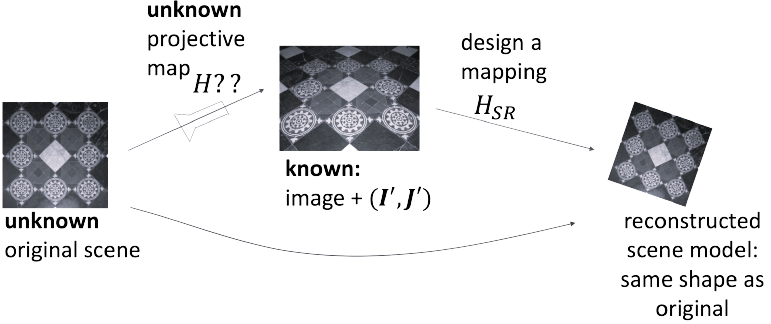
\includegraphics[width=0.75\linewidth]{images/HSR.png}
\end{figure}
The main challenges in this approach are:
\begin{itemize}
    \item Finding the projective transformation $\mathbf{H}_\text{SR}$ that restores the points $\mathbf{I}^\prime$ and $\mathbf{J}^\prime$ to $\mathbf{I}$ and $\mathbf{J}$. 
    \item Determining the vanishing line in the image to aid in finding the circular points.
\end{itemize}

\subsection{Projective transformation determination}
Finding the projective transformation $\mathbf{H}_\text{SR}$ that maps $\mathbf{I}^\prime$ and $\mathbf{J}^\prime$ back to $\mathbf{I}$ and $\mathbf{J}$ is equivalent to solving for one of the infinitely many matrices that satisfy:
\[\begin{cases}
    \mathbf{H}_\text{SR}\mathbf{I}^\prime=\mathbf{I} \\
    \mathbf{H}_\text{SR}\mathbf{J}^\prime=\mathbf{J}
\end{cases}\]
This task is non-trivial, but it can be simplified by leveraging additional geometric information, such as the degenerate conic dual to the circular points.

The degenerate conic dual to $\mathbf{I}^\prime,\mathbf{J}^\prime$ is given by:
\[\mathbf{C}_{\infty}^{\prime\ast}=\mathbf{I}^\prime \mathbf{J}^{\prime T}+\mathbf{J}^\prime \mathbf{I}^{\prime T}\]
This conic is the image of the original conic dual to the circular points $\mathbf{I}$ and $\mathbf{IJ}$, denoted by:
\[\mathbf{C}_{\infty}^\ast=\mathbf{IJ}^{T}+\mathbf{JI}^{T}\]
Since $\mathbf{C}_{\infty}^{\prime\ast}$ is the projective image of $\mathbf{C}_\infty^\ast$, any projective transformation $\mathbf{H}_\text{SR}$ that restores $\mathbf{I}^\prime$ and $\mathbf{J}^\prime$ to $\mathbf{I}$ and $\mathbf{J}$ will also restore $\mathbf{C}_{\infty}^{\prime\ast}$ to $\mathbf{C}_{\infty}^\ast$. 
Using the transformation rule for dual conics, we have:
\[\mathbf{C}^\ast_{\infty}=\mathbf{H}_\text{SR}\mathbf{C}^{\prime\ast}_{\infty}\mathbf{H}_\text{SR}^T\]
Reversing this relationship gives:
\[\mathbf{C}_{\infty}^{\prime\ast}=\mathbf{H}_\text{SR}^{-1} \begin{bmatrix} 1 & 0 & 0 \\ 0 & 1 & 0 \\ 0 & 0 & 0 \end{bmatrix} \mathbf{H}_\text{SR}^{-T}\]

By applying singular value decomposition (SVD) to the equation above, we find that $\mathbf{H}_\text{SR}^{-1}$ and $\mathbf{H}_\text{SR}^{-T}$ are orthogonal matrices. 
This leads to: 
\[\text{SVD}\left(\mathbf{C}_{\infty}^{\prime\ast}\right)=\mathbf{U}_\perp \begin{bmatrix} 1 & 0 & 0 \\ 0 & 1 & 0 \\ 0 & 0 & 0 \end{bmatrix} \mathbf{U}_{\perp}^T\]
Thus, the solution for $\mathbf{H}_\text{SR}$ is:
\[\mathbf{H}_\text{SR} = \mathbf{U}_{\perp}^{-1}=\mathbf{U}_{\perp}^T\]
To ensure proper image rectification and scaling, the matrix $\mathbf{H}_\text{SR}$ can be adjusted to:
\[\mathbf{H}_\text{SR} = \begin{bmatrix} \frac{1}{\sqrt{a}} & 0 & 0 \\ 0 & \frac{1}{\sqrt{b}} & 0 \\ 0 & 0 & 1 \end{bmatrix} \mathbf{U}^T\]
This transformation not only maps the circular points back to their original positions but also ensures that the final image is a faithful similarity reconstruction of the scene.

\subsection{Vanishing line identification}
To determine the vanishing line, one can leverage additional information from the observed scene. 
This information helps establish several key constraints:
\begin{enumerate}
    \item \textit{Known angles between lines}: when the angles between lines in the scene are known, they provide useful constraints on the vanishing line. 
        The angle between two lines depends on the angle between their normal vectors and is independent of parameters $c_1$ and $c_2$. 
        This relationship can be expressed mathematically as:
        \[\cos\vartheta=\dfrac{a_1a_2+b_1b_2}{\sqrt{(a_1^2+b_1^2)(a_2^2+b_2^2)}}\]
        Here, $a_1$, $b_1$, $a_2$, and $b_2$ are coefficients of the normal vectors of the lines. 
        This expression can be rewritten as:
        \[\cos\vartheta=\dfrac{\mathbf{l}^T\mathbf{C}_{\infty}^\ast \mathbf{m}}{\sqrt{(\mathbf{l}^T\mathbf{C}_{\infty}^\ast \mathbf{l})(\mathbf{m}^T\mathbf{C}_{\infty}^\ast \mathbf{m})}}\]
        The equation can be further simplified using the relationship $\mathbf{C}_{\infty}^\ast=\mathbf{H}^{-1}\mathbf{C}_{\infty}^{\ast\prime}\mathbf{H}^{-T}$, allowing us to express $\mathbf{l}^T\mathbf{C}_{\infty}^\ast \mathbf{m}$ as $\mathbf{l}^{\prime T}\mathbf{C}_{\infty}^{\ast\prime}\mathbf{m}^\prime$. 
        Thus, the equation becomes:
        \[\cos\vartheta=\dfrac{\mathbf{l}^{\prime T}\mathbf{C}_{\infty}^{\ast\prime}\mathbf{m}^\prime}{(\mathbf{l}^{\prime T}\mathbf{C}_{\infty}^{\ast\prime}\mathbf{l}^\prime)(\mathbf{m}^{\prime T}\mathbf{C}_{\infty}^{\ast\prime}\mathbf{m}^\prime)}\]
        In this case, $\mathbf{m}^\prime$ and $\mathbf{l}^\prime$ are derived from the image. 
        Since the angle $\vartheta$ is known, this equation provides a linear constraint on $\mathbf{C}_{\infty}^{\ast\prime}$. 
        When the lines are perpendicular ($\cos\vartheta=0$), this constraint is particularly useful.
        The unknown matrix $\mathbf{C}_{\infty}^\prime$ is symmetric, homogeneous, and singular, providing four independent constraints.
    \item \textit{Known objects shapes}: f the shape of objects in the scene is known, the reconstruction matrix $\mathbf{H}_\text{SR}$ can be determined. 
        This transformation matrix is defined as:
        \[\mathbf{H}_\text{SR} = \begin{bmatrix} \frac{1}{\sqrt{a}} & 0 & 0 \\ 0 & \frac{1}{\sqrt{b}} & 0 \\ 0 & 0 & 1 \end{bmatrix}\mathbf{U}^T\]
        The Euclidean-reconstructed image can then be calculated as $\mathbf{M}_S=\mathbf{H}_\text{SR} \cdot \textnormal{image}$. 
    \item \textit{Combinations of constraints}: it is also possible to combine known angles between lines and object shapes to derive additional constraints on the vanishing line. 
    \item \textit{Observation of rigid planar motion}: when observing rigid planar motion, which follows a similarity transformation, circular points remain invariant.
        The object in motion has three degrees of freedom, and both the center of rotation and the rotation angle can be derived.
        Given a transformation matrix $\mathbf{H}$, its eigenvectors provide important insights:
        \begin{itemize}
            \item Eigenvectors of $\mathbf{H}$ correspond to fixed points.
            \item Eigenvectors of $\mathbf{H}^{-1}$ correspond to fixed lines.
        \end{itemize}
        Specifically:
        \begin{itemize}
            \item Complex eigenvalues correspond to eigenvectors $\mathbf{I}^\prime$ and $\mathbf{J}^\prime$, where the phase represents the rotation angle.
            \item Real eigenvalues correspond to the eigenvector $\mathbf{O}^\prime$, representing the center of rotation.
        \end{itemize}
        The eigenvectors associated with the complex eigenvalues $e^{i\theta}$, and $-e^{i\theta}$ represent the images of the circular points.
        The eigenvector corresponding to the eigenvalue 1 gives the image of the center of rotation, $O$, while $\theta$ corresponds to the rotation angle.
        Using the relationship $\mathbf{C}_{\infty}^{\prime\ast}=\mathbf{I}^\prime \mathbf{J}^{\prime T}+\mathbf{J}^\prime \mathbf{I}^{\prime T}$, the singular value decomposition (SVD) can be applied to obtain $\text{SVD}(\mathbf{C}_{\infty}^{\prime\ast})=\mathbf{UC}_{\infty}^\ast \mathbf{U}^T$, where $\mathbf{U}^T$ is the rectification matrix. 
        There are two primary methods to address this:
        \begin{itemize}
            \item \textit{Direct method}: first compute $\mathbf{C}_{\infty}^{\ast\prime}$, and then derive the rectification matrix $\mathbf{H}_{\text{rect}}$.
            \item \textit{Stratified method}: first perform an affine reconstruction from projective to affine geometry, and then perform shape reconstruction from affine to metric geometry.
        \end{itemize}
        The stratified method can sometimes reduce numerical errors, providing more accurate results.
\end{enumerate}